\frametitle{Docking results of Ethotoin}
\begin{columns}
	\begin{column}{0.5\linewidth}
		\centering
		\vspace{-1em}
		\begin{figure}
			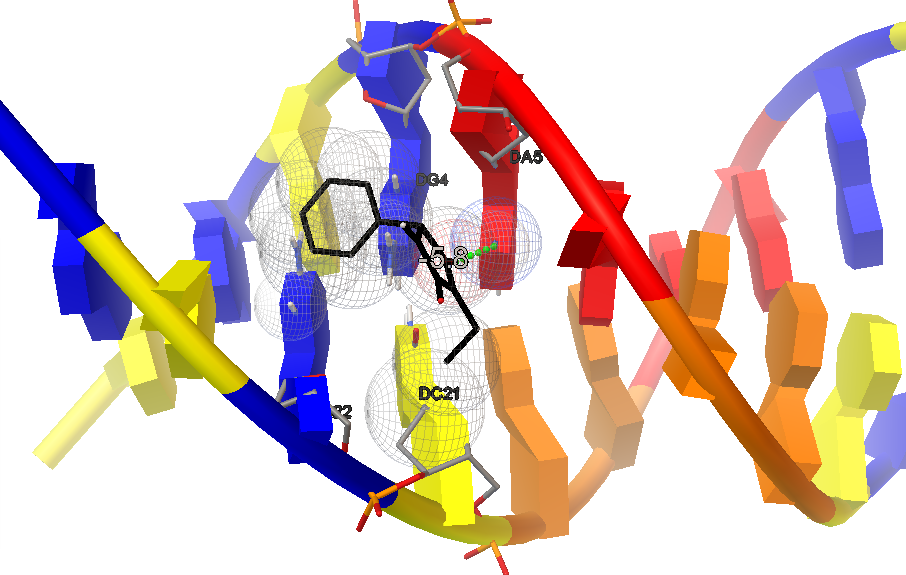
\includegraphics[width=0.7\linewidth]{ethotoin_docking_1.png}
			\caption{\centering The hydrogen bonding interaction \linebreak between Ethotoin and B-DNA.}
			\label{fig:eth_ribbon}
		\end{figure}
		\vspace{-2em}
		\scriptsize
		\begin{table}
		\tiny
		\setlength\tabcolsep{1.5pt}
		\begin{tabular}{ c | c c c } 
			\multirow{2}{7.6em}{\centering \textbf{Close interactions with B-DNA}}&\multicolumn{3}{c}{\multirow{2}{11em}{\centering DA5, DC21, DG22, DG4}}\\
			&&&\\
			\hline
			\multirow{8}{7em}{\centering \textbf{Hydrogen bonds (Angstrom Å) with B-DNA}}&\multirow{2}{6em}{\centering \textbf{Donor Atom}}&\multirow{2}{4em}{\centering \textbf{Acceptor Atom}}&\multirow{2}{5em}{\centering \textbf{Bond Length (Å)}}\\
			&&&\\
			\cline{2-4}
			&\multirow{2}{6em}{\centering H22 of DG4 (Chain A)}&\multirow{2}{6em}{\centering O2 of Ethotoin}&\multirow{2}{2em}{\centering 2.8}\\
			&&&\\
			\cline{2-4}
			&\multirow{2}{6em}{\centering H21 of DG4 (Chain A)}&\multirow{2}{6em}{\centering O2 of Ethotoin}&\multirow{2}{2em}{\centering 3.2}\\
			&&&\\
			\cline{2-4}
			&\multirow{2}{6em}{\centering H3 of DA5 (Chain A)}&\multirow{2}{6em}{\centering O2 of Ethotoin}&\multirow{2}{2em}{\centering 1.9}\\
			&&&\\
		\end{tabular}
		\caption{\centering{The close and hydrogen bonds \linebreak between Ethotoin and B-DNA.}}
		\end{table}
	\end{column}
	\hspace{-2em}
	\begin{column}{0.6\linewidth}
		\centering
		\begin{figure}
			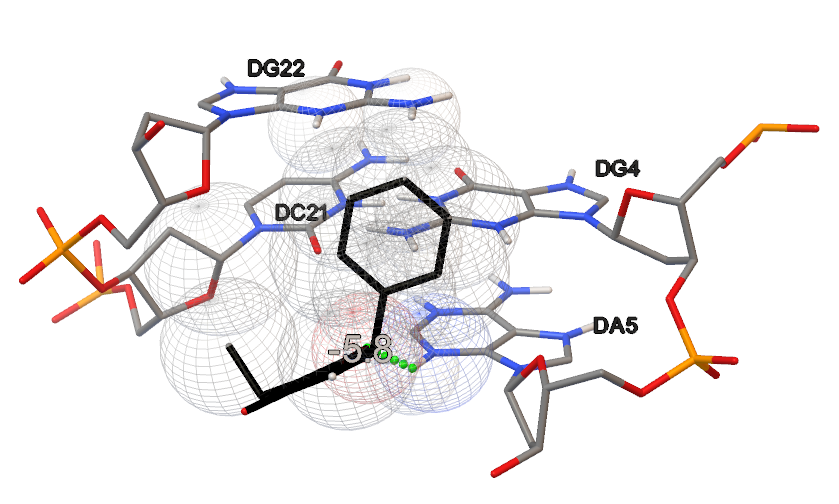
\includegraphics[width=\linewidth]{ethotoin_yakin_5.png}
			\caption{\centering The close interaction and
				binding affinity \linebreak between Ethotoin and B-DNA.}
			\label{fig:eth_close}
		\end{figure}
	\end{column}
\end{columns}